% Homework Template for Istanbul Technical University
% Prepared by [Your Full Name], Student at Istanbul Technical University
% Department of [Your Department], Course: PHYS XXX
% This LaTeX template is designed to help ITU students organize their homework submissions in a professional and structured manner.
% It provides an easy-to-read layout for mathematical computations, problem-solving, and various scientific notations.
% The template includes sections for each problem and solution, along with a title page for clear presentation.
% If you encounter any issues or need assistance with this template, feel free to contact me at (bdanis23@ku.edu.tr)
%
% Below is the detailed structure of the template including title page, sectioning, and mathematical formatting.

\documentclass[11pt]{article}
\usepackage[margin=1in]{geometry}
\usepackage{amsfonts,amsmath,amssymb}
\usepackage[none]{hyphenat}
\usepackage{fancyhdr}
\usepackage{float}
\usepackage{graphicx}
\usepackage{tikz}
\usepackage{mathdots}
\usepackage{yhmath}
\usepackage{cancel}
\usepackage{color}
\usepackage{array}
\usepackage{multirow}
\usepackage{amssymb}
\usepackage{gensymb}
\usepackage{tabularx}
\usepackage{booktabs}
\usepackage{amsmath}
\usepackage{chemfig}
\usetikzlibrary{fadings}
\usetikzlibrary{patterns}
\usetikzlibrary{shadows.blur}




\pagestyle{fancy}
\fancyhead{}
\fancyfoot{}
\fancyhead [L]{\slshape \MakeUppercase{PHYS XXX - Homework Template}}
\fancyhead [R]{\slshape Your Full Name}
\fancyfoot [C]{\thepage}
\renewcommand{\footrulewidth}{0pt}



\begin{document}
\begin{titlepage}
\begin{center}
\vspace*{1cm}
\Large{\textbf{Istanbul Technical University, XXX Department}}\\
\Large{\textbf{PHYS XXX}}\\
\vfill
\line(1,0){400}\\[1mm]
\huge{\textbf{HOMEWORK TEMPLATE}}\\[3mm]

\line(1,0){400}\\
\vfill
Your Full Name \\
090XXXXXX\\
\today\\
\end{center}
\end{titlepage}


\section*{Part 1}

\subsection*{Quesiton 1}

Compute the flux through the unitary radius sphere centered at the
coordinate origin, of the different gravitational fields:\\\\
F = x $\vec{i}$ + x $\vec{j}$ + x $\vec{k}$\\\\
F = $\frac{4y}{\sqrt{1-x^{2}}} \hspace{0.1cm} \vec{j}$

\subsection*{Solution of Quesiton 1}


for the field  F = x $\vec{i}$ + x $\vec{j}$ + x $\vec{k}$\\\\

We use divergence theorem: 

$$\iint F.dS = \iiint \nabla \cdot F \hspace{0.1cm} dV $$

$$\iint (x \vec{i} + x \vec{j} + x \vec{k}).dS = \iiint \nabla \cdot (x \vec{i} + x \vec{j} + x \vec{k})  dV . $$

If we take the divergence ; 
$$\left( \frac{\partial}{\partial x} , \frac{\partial}{\partial y } ,\frac{\partial}{\partial z} \right) \cdot \left( x \vec{i} + x \vec{j} + x \vec{k} \right) = \left( \frac{\partial x }{\partial x}  + \hspace{0.1cm} \frac{\partial x }{\partial y }  + \frac{\partial x }{\partial z} \hspace{0.1cm}  \right) = 1  $$

surface integral would be the volume of unitary radius sphere.

$$\iint (x \vec{i} + x \vec{j} + x \vec{k}).dS = \iiint 1  dV $$

$$\iiint 1  dV = \int_{0}^{1} \int_{0}^{2\pi} \int_{0}^{pi} \rho^{2} \sin\phi \hspace{0.1cm} d\phi   \hspace{0.1cm} d\theta \hspace{0.1cm} d\rho  = \frac{4 \pi}{3} \vspace{0.1cm}$$


for the field  F = $\frac{4y}{\sqrt{1-x^{2}}} \hspace{0.1cm} \vec{j}$\\\\

The relation between surface integral and volume integral:

$$\iint \frac{4y}{\sqrt{1-x^{2}}} \hspace{0.1cm} \vec{j} .dS = \iiint \nabla \cdot \left( \frac{4y}{\sqrt{1-x^{2}}} \hspace{0.1cm} \vec{j} \right) \hspace{0.1cm} dV $$

If we take the divergence ; 
$$\left( \frac{\partial}{\partial x} , \frac{\partial}{\partial y } ,\frac{\partial}{\partial z} \right) \cdot \left( 0 \vec{i} + \frac{4y}{\sqrt{1-x^{2}}} \hspace{0.1cm} \vec{j}  + 0 \vec{k} \right) = \left(    \frac{\partial  }{\partial y }  \frac{4y}{\sqrt{1-x^{2}}}  \right) = \frac{4}{\sqrt{1-x^{2}}}  $$
surface integral is transformed to volume one.
$$ \iiint \nabla \cdot \left( \frac{4y}{\sqrt{1-x^{2}}} \hspace{0.1cm} \vec{j} \right) \hspace{0.1cm} dV = \int\limits_{-1}^{1} \int\limits_{-1}^{1} \hspace{0.2cm} \int\limits_{-\sqrt{1-x^{2}}}^{+\sqrt{1-x^{2}}} \frac{4}{\sqrt{1-x^{2}}} \hspace{0.1cm} dy \hspace{0.1cm} dx \hspace{0.1cm} dz = \int\limits_{-1}^{1} \int\limits_{-1}^{1} 8 \hspace{0.1cm} dx \hspace{0.1cm} dz = 32 $$

\subsection*{Quesiton 2}

Qui nesciunt nesciunt ut dolorem dolorum et iste consequuntur eum officiis praesentium et veritatis aperiam sed aspernatur amet. Ut nemo unde qui quam nihil ut sint voluptatem. Est itaque numquam sit soluta expedita in omnis quibusdam ut laboriosam voluptate.

\subsection*{Solution of Quesiton 2}

Sed libero provident sed quia tempore sit numquam necessitatibus ut fuga officia? Et reiciendis fugiat qui nisi omnis qui dolor natus et quia quaerat eos iste quidem. Qui doloremque eveniet sed perferendis fugit qui delectus ratione nam minima error quo mollitia corrupti quo animi voluptas.

\begin{center}
\tikzset{every picture/.style={line width=0.75pt}} %set default line width to 0.75pt        

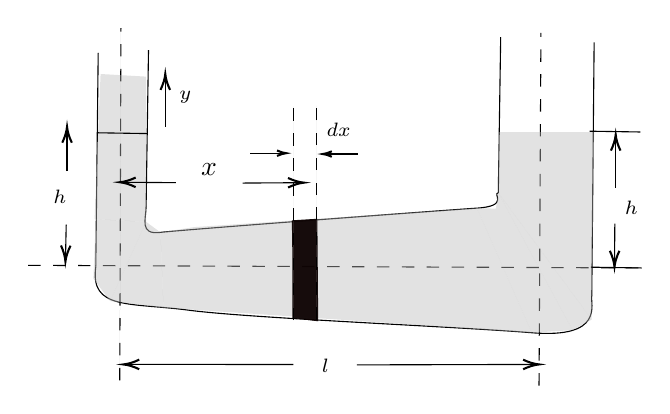
\begin{tikzpicture}[x=0.75pt,y=0.75pt,yscale=-1,xscale=1]
%uncomment if require: \path (0,273); %set diagram left start at 0, and has height of 273

%Straight Lines [id:da7612556593310547] 
\draw  [dash pattern={on 4.5pt off 4.5pt}]  (168.3,175.23) -- (463.81,176.5) ;
%Straight Lines [id:da5077535859048004] 
\draw [fill={rgb, 255:red, 186; green, 184; blue, 184 }  ,fill opacity=1 ] [dash pattern={on 4.5pt off 4.5pt}]  (212.4,230.61) -- (212.97,61) ;
%Straight Lines [id:da7130904867868506] 
\draw  [dash pattern={on 4.5pt off 4.5pt}]  (414.4,233.15) -- (415.32,63.29) ;
%Curve Lines [id:da8730989149014399] 
\draw    (200.85,175.91) .. controls (197.97,196.86) and (216.9,193.04) .. (245.75,196.86) .. controls (274.61,200.67) and (375.73,204.83) .. (410.94,207.71) .. controls (446.15,210.59) and (438.99,193.8) .. (439.8,189.9) ;
%Curve Lines [id:da5193300391786335] 
\draw    (225.09,146.65) .. controls (225.09,153.01) and (221.63,160.64) .. (232.02,159.37) .. controls (242.41,158.1) and (368.41,148.71) .. (384.48,147.68) .. controls (400.55,146.65) and (391.61,140.66) .. (394.78,140.29) ;
%Straight Lines [id:da00972128119348481] 
\draw    (202.01,72.87) -- (200.85,175.91) ;
%Straight Lines [id:da9236242736630966] 
\draw    (226.25,71.6) -- (225.09,146.65) ;
%Straight Lines [id:da20231285205109062] 
\draw    (395.93,65.24) -- (394.78,140.29) ;
%Straight Lines [id:da35498067743452966] 
\draw    (440.95,67.78) -- (439.8,189.9) ;
%Shape: Polygon [id:ds37018123167501416] 
\draw  [draw opacity=0][fill={rgb, 255:red, 185; green, 185; blue, 185 }  ,fill opacity=0.42 ] (225.09,84.32) -- (225.09,154.28) -- (200.27,153.01) -- (201.43,124.39) -- (203.16,83.05) -- cycle ;
%Shape: Polygon [id:ds8846439938078898] 
\draw  [draw opacity=0][fill={rgb, 255:red, 185; green, 185; blue, 185 }  ,fill opacity=0.42 ] (384.48,147.68) -- (410.94,207.71) -- (233.46,195.63) -- (232.02,159.37) -- (248.18,156.83) -- cycle ;
%Shape: Polygon [id:ds6352424724656798] 
\draw  [draw opacity=0][fill={rgb, 255:red, 185; green, 185; blue, 185 }  ,fill opacity=0.42 ] (439.8,189.9) -- (439.8,201.35) -- (394.78,140.29) -- (394.78,111.03) -- (440.95,111.03) -- cycle ;
%Shape: Polygon [id:ds9961413809887132] 
\draw  [draw opacity=0][fill={rgb, 255:red, 185; green, 185; blue, 185 }  ,fill opacity=0.42 ] (225.09,154.28) -- (207.78,192.45) -- (199.7,181.63) -- (200.85,153.01) -- (200.85,153.01) -- cycle ;
%Shape: Polygon [id:ds848946377082201] 
\draw  [draw opacity=0][fill={rgb, 255:red, 185; green, 185; blue, 185 }  ,fill opacity=0.42 ] (394.78,140.29) -- (430.56,206.44) -- (410.94,207.71) -- (384.48,147.68) -- (393.62,147.92) -- cycle ;
%Shape: Polygon [id:ds7787571337806549] 
\draw  [draw opacity=0][fill={rgb, 255:red, 185; green, 185; blue, 185 }  ,fill opacity=0.42 ] (439.8,201.35) -- (439.8,201.35) -- (430.56,206.44) -- (394.78,140.29) -- (439.8,201.35) -- cycle ;
%Shape: Polygon [id:ds3324742403803731] 
\draw  [draw opacity=0][fill={rgb, 255:red, 185; green, 185; blue, 185 }  ,fill opacity=0.42 ] (232.02,159.37) -- (233.46,195.63) -- (207.78,192.45) -- (225.09,154.28) -- (232.02,159.37) -- cycle ;
%Shape: Polygon [id:ds8759149779940896] 
\draw  [draw opacity=0][fill={rgb, 255:red, 11; green, 1; blue, 1 }  ,fill opacity=0.95 ] (307.6,152.8) -- (308,202.2) -- (295.6,200.6) -- (295.6,172.8) -- (295.31,153.56) -- cycle ;
%Straight Lines [id:da6226861193362436] 
\draw [fill={rgb, 255:red, 186; green, 184; blue, 184 }  ,fill opacity=1 ] [dash pattern={on 4.5pt off 4.5pt}]  (307.05,201.35) -- (307.05,98.31) ;
%Straight Lines [id:da29679456952913985] 
\draw [fill={rgb, 255:red, 186; green, 184; blue, 184 }  ,fill opacity=1 ] [dash pattern={on 4.5pt off 4.5pt}]  (296.23,201.67) -- (296.23,98.63) ;
%Straight Lines [id:da5114729545370049] 
\draw    (296,223) -- (244.72,222.98) -- (216.13,222.98) ;
\draw [shift={(214.13,222.98)}, rotate = 360] [color={rgb, 255:red, 0; green, 0; blue, 0 }  ][line width=0.75]    (7.65,-2.3) .. controls (4.86,-0.97) and (2.31,-0.21) .. (0,0) .. controls (2.31,0.21) and (4.86,0.98) .. (7.65,2.3)   ;
%Straight Lines [id:da039170308154339084] 
\draw    (326.6,223.2) -- (412.4,222.98) ;
\draw [shift={(414.4,222.98)}, rotate = 539.85] [color={rgb, 255:red, 0; green, 0; blue, 0 }  ][line width=0.75]    (7.65,-2.3) .. controls (4.86,-0.97) and (2.31,-0.21) .. (0,0) .. controls (2.31,0.21) and (4.86,0.98) .. (7.65,2.3)   ;
%Straight Lines [id:da5924445718525932] 
\draw    (450.92,155.09) -- (450.78,173.91) ;
\draw [shift={(450.76,175.91)}, rotate = 270.42] [color={rgb, 255:red, 0; green, 0; blue, 0 }  ][line width=0.75]    (7.65,-2.3) .. controls (4.86,-0.97) and (2.31,-0.21) .. (0,0) .. controls (2.31,0.21) and (4.86,0.98) .. (7.65,2.3)   ;
%Straight Lines [id:da45453081230755865] 
\draw    (451.34,137.75) -- (451.34,114.31) ;
\draw [shift={(451.34,112.31)}, rotate = 450] [color={rgb, 255:red, 0; green, 0; blue, 0 }  ][line width=0.75]    (7.65,-2.3) .. controls (4.86,-0.97) and (2.31,-0.21) .. (0,0) .. controls (2.31,0.21) and (4.86,0.98) .. (7.65,2.3)   ;
%Straight Lines [id:da9458920793070622] 
\draw    (326.94,121.61) -- (312.2,121.61) ;
\draw [shift={(310.2,121.61)}, rotate = 360] [color={rgb, 255:red, 0; green, 0; blue, 0 }  ][line width=0.75]    (4.37,-1.32) .. controls (2.78,-0.56) and (1.32,-0.12) .. (0,0) .. controls (1.32,0.12) and (2.78,0.56) .. (4.37,1.32)   ;
%Straight Lines [id:da826856323368435] 
\draw    (275.24,121.21) -- (290.55,121.21) ;
\draw [shift={(292.55,121.21)}, rotate = 180] [color={rgb, 255:red, 0; green, 0; blue, 0 }  ][line width=0.75]    (4.37,-1.32) .. controls (2.78,-0.56) and (1.32,-0.12) .. (0,0) .. controls (1.32,0.12) and (2.78,0.56) .. (4.37,1.32)   ;
%Straight Lines [id:da508596605968807] 
\draw    (271.6,135.6) -- (299.12,135.42) ;
\draw [shift={(301.12,135.4)}, rotate = 539.62] [color={rgb, 255:red, 0; green, 0; blue, 0 }  ][line width=0.75]    (7.65,-2.3) .. controls (4.86,-0.97) and (2.31,-0.21) .. (0,0) .. controls (2.31,0.21) and (4.86,0.98) .. (7.65,2.3)   ;
%Straight Lines [id:da03381315176151212] 
\draw    (239.4,135.4) -- (214.4,135.22) ;
\draw [shift={(212.4,135.2)}, rotate = 360.41999999999996] [color={rgb, 255:red, 0; green, 0; blue, 0 }  ][line width=0.75]    (7.65,-2.3) .. controls (4.86,-0.97) and (2.31,-0.21) .. (0,0) .. controls (2.31,0.21) and (4.86,0.98) .. (7.65,2.3)   ;
%Straight Lines [id:da6304211010647327] 
\draw    (186.6,155.6) -- (186.27,171.37) ;
\draw [shift={(186.22,173.37)}, rotate = 271.22] [color={rgb, 255:red, 0; green, 0; blue, 0 }  ][line width=0.75]    (7.65,-2.3) .. controls (4.86,-0.97) and (2.31,-0.21) .. (0,0) .. controls (2.31,0.21) and (4.86,0.98) .. (7.65,2.3)   ;
%Straight Lines [id:da9714260599536766] 
\draw    (187,129.8) -- (187,110.49) ;
\draw [shift={(187,108.49)}, rotate = 450] [color={rgb, 255:red, 0; green, 0; blue, 0 }  ][line width=0.75]    (7.65,-2.3) .. controls (4.86,-0.97) and (2.31,-0.21) .. (0,0) .. controls (2.31,0.21) and (4.86,0.98) .. (7.65,2.3)   ;
%Straight Lines [id:da4301882751728652] 
\draw    (201.43,111.37) -- (225.9,111.76) ;
%Straight Lines [id:da5785252500726206] 
\draw    (234.33,108.49) -- (234.33,85.05) ;
\draw [shift={(234.33,83.05)}, rotate = 450] [color={rgb, 255:red, 0; green, 0; blue, 0 }  ][line width=0.75]    (7.65,-2.3) .. controls (4.86,-0.97) and (2.31,-0.21) .. (0,0) .. controls (2.31,0.21) and (4.86,0.98) .. (7.65,2.3)   ;
%Straight Lines [id:da8079123195372362] 
\draw    (438.76,110.61) -- (463.23,110.99) ;
%Straight Lines [id:da829882866635981] 
\draw    (439.33,176.12) -- (463.81,176.5) ;

% Text Node
\draw (308.48,218.96) node [anchor=north west][inner sep=0.75pt]  [font=\scriptsize] [align=left] {$l$};
% Text Node
\draw (179.19,137.55) node [anchor=north west][inner sep=0.75pt]  [font=\scriptsize] [align=left] {$h$};
% Text Node
\draw (454.5,143.06) node [anchor=north west][inner sep=0.75pt]  [font=\scriptsize] [align=left] {$h$};
% Text Node
\draw (310.84,105.23) node [anchor=north west][inner sep=0.75pt]  [font=\scriptsize] [align=left] {$dx$};
% Text Node
\draw (239.86,90.11) node [anchor=north west][inner sep=0.75pt]  [font=\scriptsize] [align=left] {$y$};
% Text Node
\draw (250.36,125.12) node [anchor=north west][inner sep=0.75pt]   [align=left] {$x$};


\end{tikzpicture}

A galisum ratione ad quaerat reprehenderit 33 totam officiis eos dolor impedit non officiis commodi et autem quasi aut accusantium ipsa. Ut reprehenderit inventore qui voluptatem iste aut repudiandae totam id voluptas exercitationem?

Non debitis quis ut illum excepturi quo sequi assumenda sed ipsam voluptas. Aut pariatur sequi et vitae quidem et sunt itaque et facere necessitatibus?

\end{center}


\section*{Part 2}

\subsection*{Quesiton 1}

Lorem ipsum dolor sit amet. Ut recusandae sapiente sed minima voluptatem id dolor libero sed laborum molestiae. Sed quasi impedit qui facilis autem ut quia porro qui consequuntur numquam non dolores similique et tempore iure. Est dolore voluptate est numquam accusamus et consequatur asperiores ex quod sapiente non enim iusto aut iusto magni eum voluptatibus numquam. Eos quibusdam suscipit aut officia maiores ut magni ipsam sit animi accusamus ex aliquam alias ut voluptas dolores.


\subsection*{Solution of Quesiton 1}

Et laudantium autem est adipisci atque et soluta distinctio est voluptate porro est quia itaque. Et tempore fugit qui nulla autem est velit repellat ut molestiae ipsam ad tenetur voluptatem qui labore facere.

Et nemo quisquam ut tenetur enim cum unde reiciendis. Non internos repellendus ut internos molestiae a cumque iste et consectetur consectetur est nihil similique et commodi odio?

Sed reprehenderit voluptatum ut quas obcaecati et deserunt sapiente. Sit recusandae quia aut delectus praesentium ut tenetur voluptatem est quia magnam. Ut quas ducimus et aliquid similique ut omnis similique non suscipit veritatis 33 suscipit maiores qui esse saepe.

Sed eaque consequatur et nisi magni aut voluptates illo. Quo explicabo consequuntur rem quaerat consequatur qui illum inventore et possimus quos?

\subsection*{Quesiton 2}

Est provident dolores vel repellendus necessitatibus et beatae expedita eum adipisci quae sit illo sint et sint consequatur. Et amet aliquam sit nulla eveniet ut rerum dolor rem ipsum amet sed laborum quae. Est ipsum sint non similique repellendus ad voluptatibus consectetur ut iusto quas ad officiis saepe non quasi enim.

Est consequuntur quibusdam est quas galisum ut suscipit fugit sit dolorem minima 33 voluptatem officiis aut fugiat odio? Aut nesciunt fugiat et necessitatibus quasi sed voluptas saepe.

\subsection*{Solution of Quesiton 2}

Est internos velit sed odio nemo et omnis libero ab placeat libero. Ea quod consequatur eum impedit saepe sit quas nemo et fuga sint et nihil dolores ut esse error. Aut dolorem numquam sit quidem eius eos galisum deserunt 33 magnam rerum. Vel iste sint qui perspiciatis quasi vel temporibus rerum sit accusamus aspernatur.

\section*{Part 3}


\subsection*{Quesiton 1}

Nam deserunt impedit et provident deleniti eos accusantium maxime aut labore sunt est odio autem in rerum galisum. Ut itaque deleniti qui perspiciatis distinctio aut laborum dicta sed laborum exercitationem sed debitis facere eum consequatur atque? Qui voluptate mollitia non perspiciatis praesentium ex voluptas ducimus. 33 Quis eveniet et dicta ipsum qui corporis quia quo dolorum ducimus eum adipisci quibusdam qui voluptatem eveniet ad quas molestias.

Et voluptas libero nam excepturi velit sit totam impedit. Et inventore expedita sed inventore voluptas ad impedit illo? Ut pariatur ipsam 33 necessitatibus fugiat aut ducimus tempora. Non quaerat modi et iste ipsa est sequi perspiciatis.

\subsection*{Solution of Quesiton 1}

Eos omnis dolorem eum culpa molestias aut delectus alias vel voluptatem quisquam eum commodi similique cum minus saepe non rerum maxime. Et doloremque omnis et fuga quia ut eveniet molestias! Sit sunt numquam est blanditiis delectus qui nobis quisquam ad blanditiis molestiae.

Non veniam fuga et corrupti dolorum qui voluptate minus et beatae iure ea quod dignissimos. Non atque impedit est nobis debitis est error eveniet aut officiis nemo quo tenetur voluptates eos asperiores omnis cum quos corporis. Quo asperiores dolore 33 doloribus tempora ut perspiciatis molestias ut natus deleniti. Aut architecto dolor vel veniam internos quo galisum corrupti.

Aut iusto tempore aut quidem rerum a explicabo voluptatum! Aut vitae consequatur qui atque doloremque et vero error et voluptas commodi vel eligendi fuga ea totam illo id sint nesciunt.

Ut dignissimos iure At iste libero et deserunt galisum in amet voluptatum et nihil galisum. Et modi explicabo qui dignissimos officia et amet nulla qui itaque neque! Est perferendis modi eos provident excepturi eum velit pariatur. Et natus obcaecati non molestias autem qui enim molestiae qui obcaecati soluta et consequatur enim et maxime veritatis.

Aut consequatur maxime cum reprehenderit eligendi ut quisquam quidem. Quo minima repellendus vel error consequatur non incidunt galisum ab internos modi et veniam eveniet! Non autem internos ut tempore libero quo quibusdam aspernatur est sint blanditiis aut asperiores quia qui dolores doloremque. Et similique provident sit atque rerum et iusto architecto ea asperiores obcaecati hic quod culpa et quas dolore non culpa molestiae!

\subsection*{Quesiton 2}

Qui molestias deserunt qui quos aperiam et quod facere nam mollitia quaerat nam doloremque neque. Est veritatis fuga a voluptas quam in unde animi quo eaque recusandae est facilis perferendis At iure soluta. 33 aliquid accusantium a inventore nihil 33 aliquam quam et sunt architecto.

\begin{figure}[h!]
  \centering
  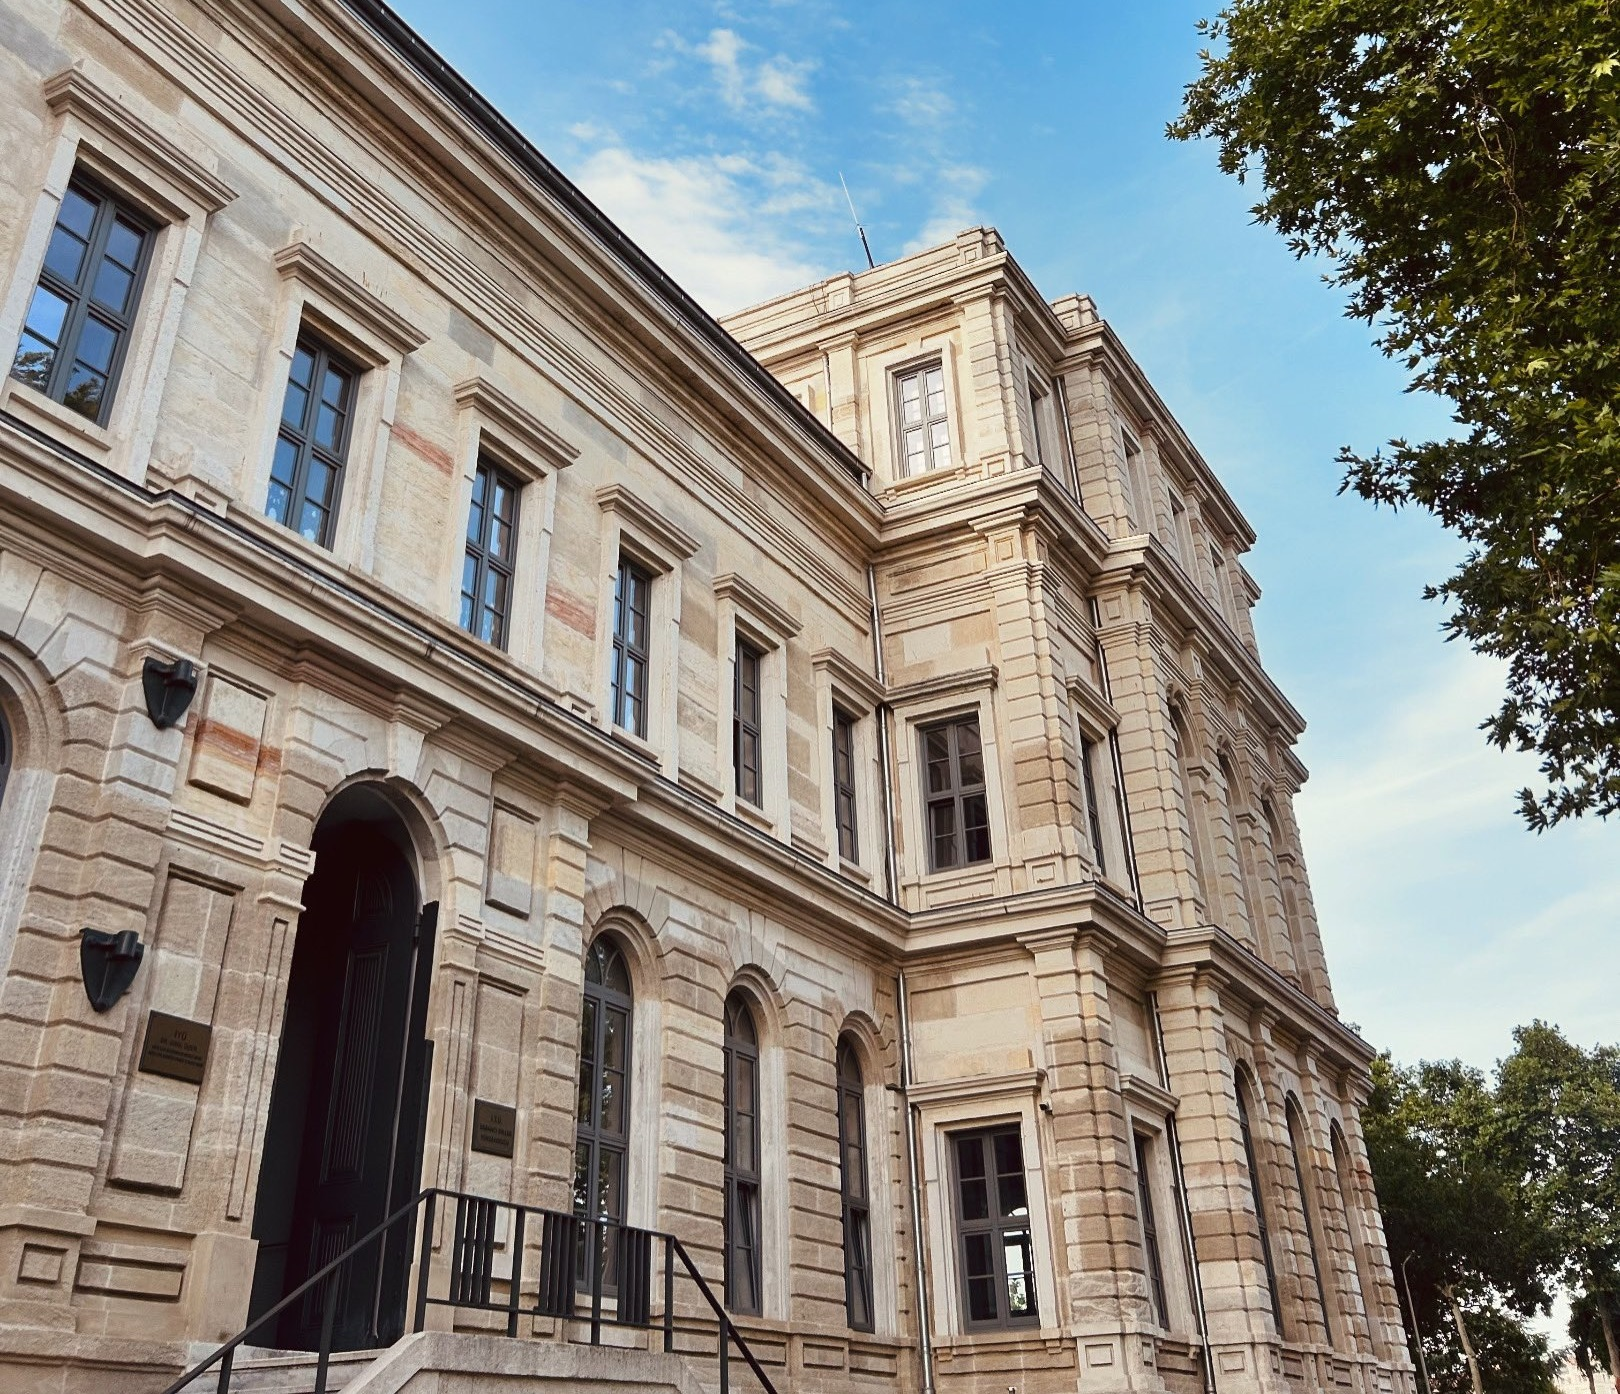
\includegraphics[width=1\linewidth]{figures/itu_example_photo.jpg}
\end{figure}

\subsection*{Solution of Quesiton 2}

At minima distinctio eos eaque molestiae et sint nobis. Sit voluptas expedita aut voluptate consequatur quo ratione laboriosam non cumque consectetur sed rerum similique id soluta esse vel quisquam veritatis. In culpa fuga est galisum neque et galisum soluta sit quis fugit ab ratione nihil et culpa galisum.

Et quaerat iste et quae delectus a quasi ipsum qui fuga explicabo eos deleniti atque aut impedit sunt ut sunt quod. Ut quasi corrupti qui laborum totam est animi omnis ut quam excepturi ea natus quae. Et velit omnis qui dolorem praesentium et enim animi et alias libero sit vitae amet et ullam ducimus.

Est cumque fugit in aliquid nihil sit error facilis! Ut vitae possimus ut atque debitis a temporibus eligendi et consequuntur vitae rem quia tenetur et omnis magni ut distinctio voluptatem. Et repudiandae temporibus ut voluptates debitis ea doloremque sunt 33 laborum aspernatur.

\end{document}


